\documentclass{homework}

\usepackage{mathtools}
\usepackage{amsmath}
\usepackage{amsfonts}
\usepackage{amssymb}

\author{Michael D. Walker (mw6136)}
\class{COS597E: Programming Languages, Distributed Systems}
\date{\today}
\title{Final Project Proposal: \\ Dynamic Load Balancing in a Massively Parallel Reacting Flow Solver}

\begin{document} \maketitle
\section{\textbf{Introduction}}
\noindent Modern Computational Fluid Dynamics (CFD) software relies on distributed-memory parallel computer architectures for large-scale computations. Using resources efficiently while at the same time maintaining high accuracy of the numerical solution is a major challenge. \emph{Computational load imbalance} is a well-known performance issue in multiprocessor reacting flow (e.g., combustion) simulations utilizing directly integrated chemical kinetics. \noindent \textbf{This project proposes to implement a \emph{dynamic load balancing} scheme (specifically Lend When Idle) on my research group's (lab: \href{https://ctrfl.princeton.edu/}{CTRFL}) low Mach number flow solver, \texttt{NGA} \cite{DESJARDINS2008,MACART2016}}. Additionally this project proposes to develop a \emph{reference mapping} paradigm to sort group cells with similar thermochemical composition, thereby evaluating their chemical source terms only when sufficiently dissimilar.
\section{\textbf{Background}}
\noindent \texttt{NGA} is a 3-D finite-difference energy-conserving incompressible flow solver, capable of solving the variable-density Navier-Stokes equations on structured Cartesian meshes using a fractional-step method. It was written for massively parallel large-eddy simulation (LES) and direct numerical simulation (DNS) of both premixed and non-premixed reacting turbulent flows. It is parallelized using a hybrid \texttt{MPI}/\texttt{OpenMP} approach and is highly scalable. \texttt{NGA} uses an operator splitting technique to decouple the conservation equations and chemical source term calculations. With this technique, chemistry can be treated as an independent stiff ordinary differential equation (ODE) system within each computational cell. \texttt{NGA} then uses \texttt{SUNDIALS} \cite{SUNDIALS} (SUite of Nonlinear and DIfferential/ALgebraic equation Solvers) \texttt{CVODE} (unsteady solver) for solving stiff systems of initial value ODEs for detailed chemistry (chemical Jacobian construction, inversion, and Newton iteration). 
\\ \\ \noindent
Typically, the computational cost of the chemical source term evaluation dominates the performance metrics and creates an un-even computational load distribution in parallel applications. This is discussed in more detail in \hyperref[appendixA]{Appendix A}, and furthermore chemical Jacobian evaluation and factorization is the most expensive step in combustion simulations. Load balancing is not handled internally by the \texttt{SUNDIALS} integrators but rather is the responsibility of the application developer. As a result of the highly non-linear characteristics of chemical kinetics, a large variation in the convergence rates of the ODE integrator may occur, leading to a high load imbalance across multiprocessor configurations. However, the independent nature of chemistry ODE systems leads to a problem that can be parallelized easily (embarrassingly parallel) during the flow solution. The presented model takes advantage of this feature and balances the chemistry load across available resources.

\section{\textbf{Systems Component: Dynamic Load Balancing}}
\noindent Lend When Idle \cite{LeWI_ICPP09,GARCIA2014,DLB_OpenMP_SMPS} (LeWI) is a novel \emph{work stealing} \cite{Work_Stealing} algorithm that distributes resources equally among \texttt{MPI} processes in a node while they are doing computation, and re-assigns resources of \texttt{MPI} processes while they are blocked in communication calls. One of its main properties is that the load balancing is task neutral, done at runtime without analyzing nor modifying the application previously.
\\ \\ \noindent
This will be implemented for the \texttt{NGA} combustion subroutine \texttt{combustion.f90}, which is the most poorly balanced. For the reasons discussed in \hyperref[appendixA]{Appendix A}, chemical Jacobian construction, factorization, and inversion occurs in this subroutine, so it is also the most costly. LeWI will then be implemented in as many other subroutines as time permits (e.g., boundary condition enforcement \texttt{borders.f90} and mesh discretization \texttt{geometry.f90}). 

\section{\textbf{Programming Languages Component: Reference Mapping}}
\noindent The timestep value and hence the total number of floating-point operations during the integration depends on the initial thermochemical composition. Parallelization is achieved with geometrical domain decomposition, leading to explicit chemistry load imbalance due to spatially and temporally varying values. A simple reference mapping feature will allow a further reduction in computational cost. This approach groups cells sharing similar thermochemical composition values together and solving the chemistry only once for this group \cite{DLBFoam_1}. Such a mapping approach is intended to be used for regions with low reactivity, (e.g., where no fuel is present or in low-temperature regions far upstream and downstream of the flame, where few chemical reactions are occurring). \textbf{The reference mapping acts as a filter for load balancing, where the reaction rates of cells satisfying a user-given criteria are copied from a reference cell solution.} At a given time instance, a reference cell is picked and the chemistry source term of that cell is solved and copied to other reference cells. The criteria used for identifying the reference cells is: $Z_i < Z_\textrm{tol}$, $|T_i - T_\textrm{ref} | < T_\textrm{tol}$, where $Z_i$ and $T_i$ are mixture fraction (the mass fraction of fuel in a fuel/oxidizer stream) and temperature of $i$-th cell, respectively, $T_\textrm{ref}$ denotes the temperature of the chosen reference cell and $Z_\textrm{tol}$ and $Z_\textrm{tol}$ are the user-defined tolerance values, specified in the \texttt{input} and \texttt{config} files. 
\\ \\ \noindent
Implementing this approach requires additional pairing between \texttt{NGA} combustion subroutine \texttt{combustion.f90} and mesh grouping subroutine \texttt{geometry.f90}. As long as properly strict tolerances are used (chemical reactions are highly non-linear based in an Arrhenius law), the introduced error should be rather small and not affect the global characteristics of the reactive simulation. The reference mapping model should improve the balancing performance modestly by further reducing the load of the more idle processes and increasing their potential to receive more load from the busier processes. 

%The PL component of this project would be to implement this scheme with both \texttt{OpenMP} and \texttt{SMPSuperscalar} protocols at the inner layer of parallelism (this has already been done by the original authors \cite{DLB_OpenMP_SMPS}). \texttt{OpenMP} can only change the number of threads outside a parallel region (e.g., ``DO'' loop). This means that when an \texttt{MPI} process lends its CPUs the \texttt{MPI} process that wants to use them is not able to do so until reaching a new parallel region. This limitation makes the performance of the algorithm highly dependent on the number of parallel regions that the application presents between \texttt{MPI} blocking calls (i.e., if there is just one parallel loop between \texttt{MPI} blocking calls we cannot change the number of threads, therefore, the application cannot be balanced). Conversely, \texttt{SMPSuperscalar} is a shared memory programming model that allows for the change of the number of threads at any time. I would compare the performance differences, discuss ease of implementation, and other considerations.

\section{\textbf{Performance Evaluation}}
\noindent \texttt{NGA} currently uses a rudimentary load balancing scheme by approximating the work for each cell ahead of time by tracking the work required to integrate the previous timestep. Thus, it is in the earliest timesteps that more robust load balancing scheme could provide considerable speedup.
\\ \\ \noindent
Several test cases will be used to evaluate performance. First, to verify proper code execution a fully-developed turbulent pipe flow configuration (presented in \hyperref[appendixC]{Appendix C}) will be simulated. This case has previously been used to conduct weak scaling studies of \texttt{NGA} with increasing grid resolution. More detailed performance benchmark test cases would be simulated using Large Eddy Simulation data of a hydrogen jet flame \cite{TNF,BARLOW1994,BARLOW1996} and Sandia Flame D \cite{BARLOW1998}. Such simulations were published\cite{LACEY2021} using \texttt{NGA} without load balancing (note the massive time per timestep for the early timesteps of Figures 4 and 5 therein).

\section{\textbf{Proposed Timeline}}
\noindent Project Milestones:
\begin{itemize} \small
\item By 22OCT (Survey deadline), complete literature review, explore existing load balancing libraries. Gain better understanding of \texttt{geometry.f90} subroutine in \texttt{NGA} to implement reference mapping.
\item By 12OCT (Progress Report deadline), implement LeWI on \texttt{combustion.f90}. Demonstrate code execution on annulus pipe flow test case.
\item By 25NOV, implement reference mapping with proper modifications to \texttt{input} and \texttt{config}. Plan to have large jobs ready to submit to \texttt{TIGER} and \texttt{PERLMUTTER} clusters over Thanksgiving break. Ideally the jet flame benchmark tests, if not, then an annulus pipe flow scaling study up to $2^{14}$ cores.
\item Analysis and figure generation until class presentation.
\item By 05DEC, complete project presentation. Continue detailed benchmark tests if not completed.
\item By 11DEC, complete Final Report.
\end{itemize} \normalsize

\noindent Timeline mitigations to ensure a deliverable project by the end of the course:
\begin{itemize} \small
\item Implement LeWI only on the \texttt{combustion.f90} subroutine, rather than all core subroutines of \texttt{NGA}.
\item Simulate only the Annulus Pipe Flow test case and conduct an associated scaling analysis, rather than simulating the more complex benchmark cases.
\end{itemize}\normalsize

\section{\textbf{Personal Benefits}}
\noindent This project would directly benefit my academic research and those of my collaborators (the Computational Turbulent Reacting Flow Laboratory, \href{https://ctrfl.princeton.edu/}{CTRFL}), by potentially considerably improving the performance of our group's primary flow solver.  There is ongoing work utilizing In-Situ Adaptive Tabulation (ISAT) \cite{LACEY2021} to improve memory allocation and retrieval. The proposed project would integrate nicely with that effort to potentially generate publishable results.

\bibliographystyle{unsrt}
\bibliography{citations}
\newpage
\appendix
\section{\textbf{Numerical Scheme and Load Imbalance in Reacting Flow Solvers}} \label{appendixA}
\noindent \texttt{NGA} \cite{DESJARDINS2008,MACART2016} is a 3-D finite-difference energy-conserving low-Mach number flow solver, using derivative operators of arbitrarily high order. It is capable of solving the variable-density Navier-Stokes equations on structured meshes using a fractional-step method. Spatial discretization errors are reduced using local $(n-1)$-th order Lagrange polynomial interpolation to achieve $n$-order accurate viscous terms. The code utilizes detailed temperature- and composition-dependent transport and thermodynamic properties, detailed chemical kinetics, and an ideal gas equation of state. \texttt{NGA} was written for massively parallel large-eddy simulation (LES) and direct numerical simulation (DNS) of both premixed and nonpremixed reacting turbulent flows. It is parallelized using a hybrid \texttt{MPI}/\texttt{OpenMP} approach and is highly scalable. \texttt{NGA} uses an operator splitting technique to decouple the conservation equations and chemical source term calculations. 
\\ \\ \noindent
A linear or non-linear system can be defined in matrix form as $\Phi \equiv \phi_{i,j} $ and $\mathbf{f}(\Phi) \equiv f_{i,j} (\Phi)$ for $ i= 1, \dots, N $, $ j= 1, \dots, N $. Parallelization is achieved with geometrical domain decomposition. The Strang splitting scheme is achieved with the spatially discretized governing equations:
$$\frac{\textrm{d} \Phi}{\textrm{d} t} = \underbracket[0.5pt]{\mathbf{T}(\Phi)}_{\textrm{transport}} + \underbracket[0.5pt]{\mathbf{S}(\Phi)}_{\textrm{chemistry}} $$
The time derivative is approximated by finite difference involving
the current and future values. The gradient and divergence operators are approximated with linear functions involving multiple neighboring cells. Transport is relatively linear and has a highly structured Jacobian, with weak coupling between species. Chemistry is highly nonlinear and typically solved implicitly. Chemistry terms are local, so each mesh volume can be solved independently (i.e., in parallel). The chemistry and transport substeps are then:
\scriptsize
\begin{alignat*}{3}
    \frac{\textrm{d} \Phi}{\textrm{d} t} &= \mathbf{S}(\Phi^{(1)}), \qquad &&\Phi^{(1)}(x,0) = \Phi(x,t_n) \;\; & &\textrm{on} \; [t_n, t_n + \Delta t / 2] \\
    \frac{\textrm{d} \Phi}{\textrm{d} t} &= \mathbf{T}(\Phi^{(2)}), \qquad &&\Phi^{(2)}(x,0) = \Phi^{(1)}(x,\Delta t / 2) \;\; & &\textrm{on} \; [t_n, t_n + \Delta t] \\
    \frac{\textrm{d} \Phi}{\textrm{d} t} &= \mathbf{S}(\Phi^{(3)}), \qquad &&\Phi^{(3)}(x,0) = \Phi^{(2)}(x,t_n) \;\; & &\textrm{on} \; [t_n + \Delta t / 2, t_n + \Delta t]
\end{alignat*}
\normalsize
Considering the time integration of a stiff reacting system, each implicit integration step involves evaluation of the source terms by Jacobian evaluation and factorization in a Newton-Raphson scheme. A system of ODEs in chemistry is defined based on multiple chemical species $N$ (i.e., types of molecules) evolving through coupled reactions $\frac{d \Phi}{d t} = \mathbf{S} \Phi$, where $\Phi = [\phi_1, \phi_2, ... \phi_N] \in \mathbb{R}^N$ and $\mathbf{S} \in \mathbb{R}^{N \times N}$. Any time integration scheme requires the eigenvalues of $\mathbf{S}$ to lie inside the stability region of the method. The system is stiff if for the set of the eigenvalues $[\lambda_1, \lambda_2, ... \lambda_N]$ of matrix $\mathbf{S}$: $|\lambda_\textrm{max}|/|\lambda_\textrm{min}| \gg 1$
A stiff problem requires a very small timestep for stability with respect to $|\lambda_\textrm{max}|$ in conjunction with a very long time integration to see any significant change in magnitude associated to $|\lambda_\textrm{min}|$.
\\ \\ \noindent
The system $\mathbf{S}(\Phi) = 0$ is solved first by constructing the Jacobian in 2-D $\mathbb{J} \equiv \partial S_{i,j} \, / \, \partial \phi_{i,j}$. Then the Newton-Raphson scheme computes the components of the matrix. Each iteration is defined by the linear system $\mathbb{J}(\Phi^{\, n+1} - \Phi^n) = $ -$ \mathbf{S}(\Phi^n)$ and can then be solved through direct matrix inversion sequentially,
$$ \Phi^{\, n+1} = \Phi^n - [\mathbb{J}^{-1} \cdot \mathbf{S}(\Phi^n)] \quad \textrm{.} $$
Here the Jacobian is an $N^2 \times N^2$ matrix and thus \textbf{Jacobian evaluation and factorization is the most expensive step in combustion simulations}.
\\ \\ \noindent
With this technique, chemistry can be treated as an independent stiff ODE system within each computational cell. \texttt{NGA} then uses \texttt{SUNDIALS} \cite{SUNDIALS} (SUite of Nonlinear and DIfferential/ALgebraic equation Solvers) \texttt{CVODE} (unsteady solver) for solving stiff systems of initial value ODEs for detailed chemistry (chemical Jacobian construction, inversion, and Newton iteration). 
\\ \\ \noindent
Typically, the computational cost of the chemical source term evaluation dominates the performance metrics and creates an un-even computational load distribution in parallel applications. The difficulties occur due to the intrinsic and non-linear nature of the ODE system. Cost of solving the associated stiff ODEs scales quadratically with the number of species \cite{DLBFoam_1,DLBFoam_2}. Furthermore, due to the vast scale separation between the fastest and slowest chemical reaction time scales, the system of ODEs is practically always numerically stiff, requiring the use of implicit time integrators with low timestep values.
\\ \\ \noindent
Load balancing is not handled internally by the \texttt{SUNDIALS} integrators but rather is the responsibility of the application developer. As a result of the highly non-linear characteristics of chemical kinetics, a large variation in the convergence rates of the ODE integrator may occur, leading to a high load imbalance across multiprocessor configurations. However, the independent nature of chemistry ODE systems leads to a problem that can be parallelized easily (embarrassingly parallel) during the flow solution. The presented LeWI model takes advantage of this feature and balances the chemistry load across available resources.
\\ \\ \noindent
Because the ODEs are uncoupled across the domain, there is considerable freedom in staging their integration. In multi-threaded CPU-based implementations, the total work to integrate all the cells in the domain can be distributed arbitrarily across the available threads with no race or synchronization concerns. The work for each cell can be approximated ahead of time by tracking the work required to integrate the previous timestep. Thus, it is in the earliest timesteps that a Lend When Idle scheme could provide considerable speedup. (Note that unlike the examples \cite{AMReX,PeleC,PeleMP} presented in the \texttt{SUNDIALS} paper, \texttt{NGA} does not have adaptive mesh refinement, so it should be a simpler implementation.)

\section{\textbf{Computational Resources}}\label{appendixB}
\noindent
Computational facilities managed by Princeton University and the Department of Energy (DOE) will be used as part of the proposed project. These computational resources are adequate for moderate-scale Direct Numerical Simulation (DNS) and Large Eddy Simulation calculations at lower Reynolds numbers, and all data post-processing. For larger-scale DNS calculations at higher Reynolds numbers, external computational resources are available through the DOE Computational Science Graduate Fellowship allocation.
\\ \\
\noindent
\texttt{TIGER} \cite{TIGER} is a HPE Apollo cluster comprised of 408 Intel Skylake CPU nodes (2 sockets per node). There are 16,320 processors available (40 per node). Each node contains at least 192 GB of memory (4.8 GB per core). There are also 40 nodes with memory of 768 GB (19 GB per core). Every 40-core node is interconnected (24 nodes per chassis) by a Omnipath fabric with oversubscription. Managed by the Princeton Institute for Computational Science and Engineering (PICSciE).
\\ \\
\noindent
\texttt{PERLMUTTER} \cite{PERLMUTTER} is a HPE Cray EX (Shasta) platform, a heterogeneous system of 3,072 CPU-only and 1,792 GPU-accelerated nodes. On the CPU partition, each node each contains two AMD EPYC 7763 (Milan) processors. Every 64-core node has 8 GB of memory per core and is interconnected by one HPE Slingshot 11 NIC (200G $+$ 25 GB/s bandwidth with PCIe 4.0 NIC-CPU connection). The CPU partition achieves performance of 7.7 PFLOPS aggregate peak FP64 and 1536 TB aggregate memory. Managed by the Lawrence Berkeley National Laboratory National Energy Research Scientific Computing Center (NERSC).

\section{\textbf{Scaling of NGA and Benchmark Problem: Annulus Pipe Flow}} \label{appendixC}
\begin{figure}[h!]
    \centering
    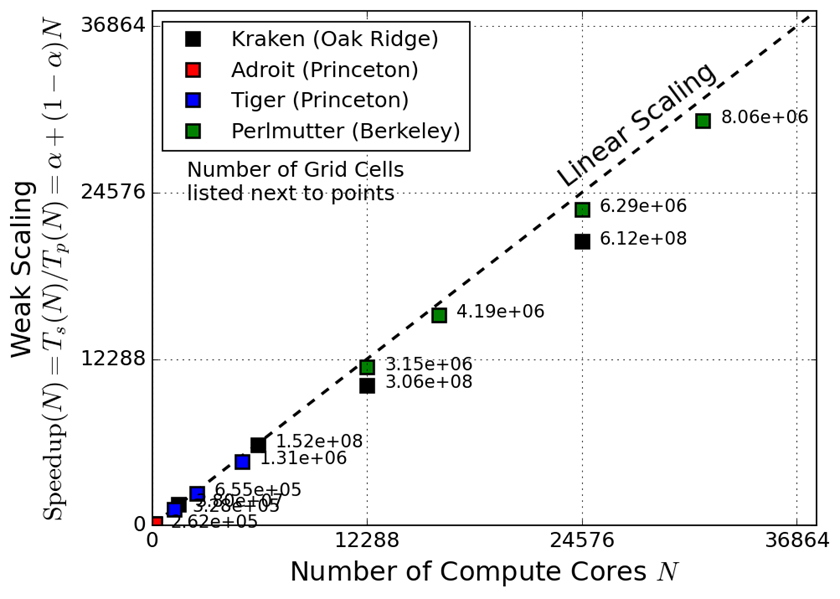
\includegraphics[width=0.6\linewidth]{NGA_scaling.png}
    \caption{NGA exhibits excellent scale-up characteristics. The largest run so far consisted of over 1.6 billion cells, and almost 50,000 compute cores.}
    \label{fig:Scaleup2}
\end{figure}
\noindent A weak scaling study of \texttt{NGA} can be conducted using the following simulation of fully developed flow in a pipe and surrounding annulus. The fluid properties correspond to methane in the pipe and air in the annulus. An initial velocity profile is specified, but over time the flow transitions to turbulent and becomes fully developed because a periodic boundary condition is used in the axial $x$ direction.
\\ \\ \noindent
A scaling study can be conducted by increasing the grid resolution and number of processors while maintaining $\sim 256$ cells per core. Also below is a sample \texttt{slurm} script for submitting the job to the scheduler on \texttt{TIGER}. It is configured to run the job on 80 processors (2 nodes, 40 cores each). In the \texttt{NGA} input file, it is specified that the domain will be split into 8 segments in the y (radial) direction, and each segment will be computed on four processors using \texttt{OpenMP}. 
\small
\begin{verbatim}[language=Fortran]
# INITIALIZATION PARAMETERS ########################
! Name
Simulation :		pipe
! Parameters
nx :			64
nz :			64
Length :		0.04
! Pipes definition
ny :			64	64
Radius :		0.0	0.00225
			0.002	0.00375
Stretching :		2.0	2.0
! Initial velocity field
Mean U Velocity :	67.0	59.5 
Mean W Velocity :	0	0
Laminar initial flow :	0	0
Fluctuation rel. amp. :	0.2	0.2
! Files
Init config file :	config
Init data file :	data.0
# RUNNING PARAMETERS ###############################
! Files
Configuration file :    config
Data file to read :     data.0
Data file to write :    data.1
Data frequency :        1e-4 
Optional data to read : optdata.0
Optional data to write: optdata.1
! Inflow file to write :	inflow.mz.v57
! Inflow frequency :      0.1e-6
! Inflow location :       0.04
! Notes
! 0 -> 1 : running simulation on 32 processors
! Partitioning
Processors along X :    5
Processors along Y :    4
Processors along Z :    1
OpenMP threads :	4
! Properties            methane         air @ 300K
Chemistry model :       none
Density :		0.651635	1.17214
Viscosity :		1.14597e-5	1.86344e-5
Diffusivity :           0		0
Temperature :           0		0
! Subgrid Scale model
Use SGS model :         .true.
SGS averaging :         Lagrangian
SGS Override Lag. :     .true.
! Body forces
Gravity :		-9.8067	0.0	0.0
! Time advancement
Timestep size :         0.5e-6
CFL number :            2
Subiterations :         2
! End of simulation
Maximum iterations :    5000
Maximum time :          100000
Maximum wall time :     1.0
! Velocity
Velocity conv scheme :	2
Velocity visc scheme :	2
Implicit directions :	xyz
! Pressure
Pressure solver :	bicgstab
Pressure fft :		.true.
Pressure precond :	tridiag
Pressure cvg :		1.E-7
Pressure iterations :	1
! Output
Output type :           ensight-3D
Output frequency :      2e-5
! Statistics
Statistics type :	1D-y
Statistics locations x:	all
Statistics frequency :	5e-5
\end{verbatim}
\newpage
\begin{verbatim}[language=Fortran]
#!/bin/bash
# HEADER for Parallel job using 80 processors:
#SBATCH --nodes=2               # number of nodes
#SBATCH --ntasks-per-node=10    # number of processors per node
#SBATCH --cpus-per-task=4       # number of cpus per task
#SBATCH -t 1:00:00              # run for 1 hr max
#SBATCH --mail-type=begin       # send email when process begins...
#SBATCH --mail-type=end         # ...and when it ends...
#SBATCH --mail-type=fail        # ...or when it fails.
#SBATCH --mail-user=your_email@princeton.edu    # send notifications to this email
#SBATCH -e job.err              # Name of output file for error messages
#SBATCH -o job.out              # Name of output file for standard output

# BODY - commands to be run
# Load required modules
module load intel               
module load intel-mpi

# Set number of openmp threads and number of MPI tasks
export OMP_NUM_THREADS=$SLURM_CPUS_PER_TASK
export NTASKS=$(echo "$SLURM_NNODES*$(echo $SLURM_TASKS_PER_NODE | cut -d '(' -f 1)" | bc -l)

echo $OMP_NUM_THREADS
echo $NTASKS

# Print some information
echo Directory is `pwd`
echo Time is `date`
echo
echo This job runs on the following processors:
echo $SLURM_JOB_NODELIST
echo This job has allocated $SLURM_NNODES nodes with $SLURM_TASKS_PER_NODE cores per node.
echo

# run arts
srun -n $NTASKS ~/NGA/bin/arts input_pipe
\end{verbatim}

\end{document}